\chapter{Wyniki eksperymentów}
\thispagestyle{chapterBeginStyle}

W tym rozdziale przyjrzymy się wynikom przeprowadzonych eksperymentów dla omawianych wcześniej algorytmów i ich modyfikacji. Na początku rozważymy algorytm \texttt{Streaming MinCount} - porównamy podejście naiwne, ulepszenia przedstawione w rozdziale \ref{impr_mincount} oraz metodę \textit{estymatora ważonego} dla tego algorytmu. Pokażemy również wyniki dla zaproponowanego przez nas w rozdziale \ref{diff_weighted} estymatora operacji różnicy. Następnie dla algorytmu \texttt{HyperLogLog}, skupimy się głównie na operacji przekroju - porównamy podejście naiwne, korzystające z indeksu \textit{Jaccarda} i metodę estymatora \textit{ważonego} dla tegoż algorytmu, zaprezentowaną w rozdziale \ref{hll_weighted}. %Na koniec porównamy efektywność obu algorytmów w kontekście operacji teoriomnogościowych i postaramy się określić które z nich sprawdzą się najefektywniej w praktyce. 
\AW{Nie jestem pewien czy porównywac ze soba wprost te dwa algorytmy (MinCount i HLL) - nie mam do tego jakichs sensownych eksperymentów, trzebaby je jakos zbadac przy wykorzystaniu podobnej ilosci pamieci albo cos w tym stylu - moglibysmy to pozostawic moze jako otwarta kwestię do sprawdzenia w ''przyszlosci''? Jak Pan sądzi?}

Eksperymenty przeprowadzone w tym rozdziale badają dokładność algorytmów na przestrzeni różnych indeksów \textit{Jaccarda}. Dokładność algorytmu mierzymy przez $\frac{\hat{n}}{n}$, czyli stosunek liczności zbioru wyznaczonej przez estymator do prawdziwej liczności zbioru.

\section{Wyniki dla algorytmu Streaming MinCount}
Na początek przedstawiamy wyniki dla trzech metod estymacji dla algorytmu \texttt{Streaming MinCount}:
\begin{enumerate}
	\item metoda naiwna (z \textit{zasady włączeń i wyłączeń})
	\item ulepszenia zaproponowane w rozdziałach \ref{impr_sum} oraz \ref{impr_inter}
	\item metoda \textit{estymatora ważonego}
\end{enumerate}
We wszystkich eksperymentach dla tego algorytmu, ustaliliśmy parametr $k = 100$, czyli szkice przetrzymywały 100 najmniejszych haszy.
Na wykresach przedstawiamy wartości $\frac{\hat{n}}{n}$ dla poszczególnych metod, oznaczone na legendzie przez odpowiednio:
\begin{enumerate}
	\item \textbf{err\_naive}
	\item \textbf{err\_impr}
	\item \textbf{err\_reweigh}
\end{enumerate}
Wykresy \ref{fig:KMV_2sets_inter} oraz \ref{fig:KMV_2sets_unions} przedstawiają wyniki eksperymentów dla sum i przekrojów dwóch zbiorów.

\begin{figure}[h!]
    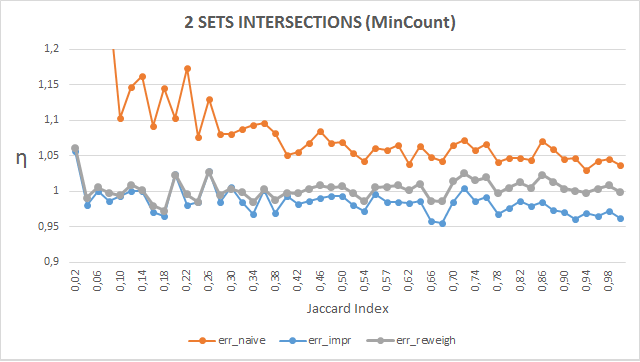
\includegraphics[width=0.6\textwidth]{KMV_2_sets_inter.png}
    \centering
    \caption{Porównanie metod dla przekrojów 2 zbiorów przy $n=10^5$}
    \label{fig:KMV_2sets_inter}
\end{figure}

\begin{figure}[h!]
    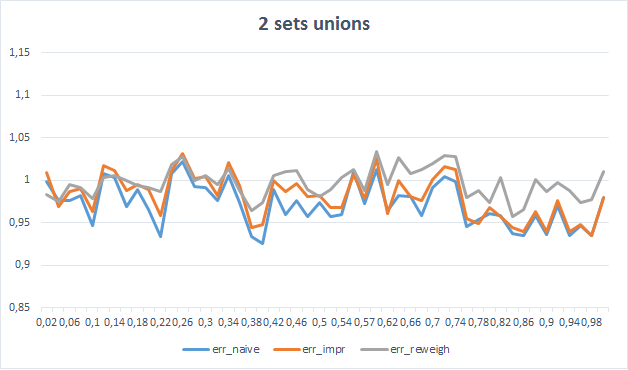
\includegraphics[width=0.6\textwidth]{KMV_2_sets_unions.png}
    \centering
    \caption{Porównanie metod dla sumy 2 zbiorów przy $n=10^5$}
    \label{fig:KMV_2sets_unions}
\end{figure}

Zauważmy, że dla operacji sumy - praktycznie na całym przedziale indeksów \textit{Jaccarda} zbiorów - najmniejszy błąd posiada metoda \textit{estymatora ważonego}. W przypadku przekroju - metody $2.$ oraz $3.$ wypadają o wiele lepiej niż metoda naiwna. Na wykresie możemy zauważyć, że metoda \textit{estymatora ważonego} posiada podobną tendencję jak metoda $2.$, ale dla większości indeksów \textit{Jaccarda} posiada mniejszy błąd.

Na kolejnych wykresach: \ref{fig:KMV_10sets_inter}, \ref{fig:KMV_10sets_unions}, \ref{fig:KMV_100sets_inter} oraz \ref{fig:KMV_100sets_unions}, zestawiliśmy wyniki dla sum i przekrojów większej liczby zbiorów. Wykonaliśmy eksperymenty dla 10 oraz 100 zbiorów o mocach $n = 10^5$, porównując metody $2.$ oraz $3.$ Metodę naiwną pominęliśmy ze względu na jej znaczące wady opisane w rozdziale \ref{naive_est}. 

Możemy zauważyć, że również jak na poprzednich wykresach dla dwóch zbiorów - metoda \textit{estymatora ważonego} posiada podobną tendencję jak metoda $2.$, ale również minimalizuje błąd - zwłaszcza dla dużych \textit{indeksów Jaccarda}.

\begin{figure}[h!]
    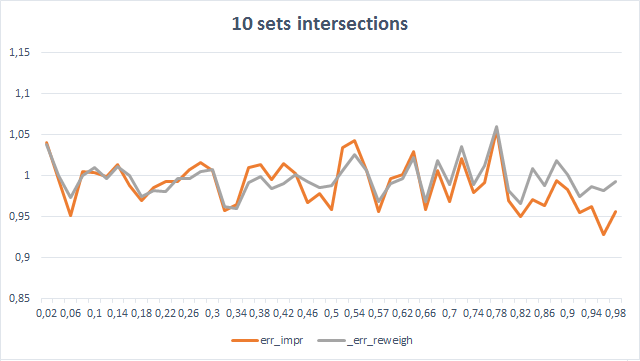
\includegraphics[width=0.6\textwidth]{KMV_10_sets_inter.png}
    \centering
    \caption{Porównanie metod dla przekroju 10 zbiorów}
    \label{fig:KMV_10sets_inter}
\end{figure}

\begin{figure}[h!]
    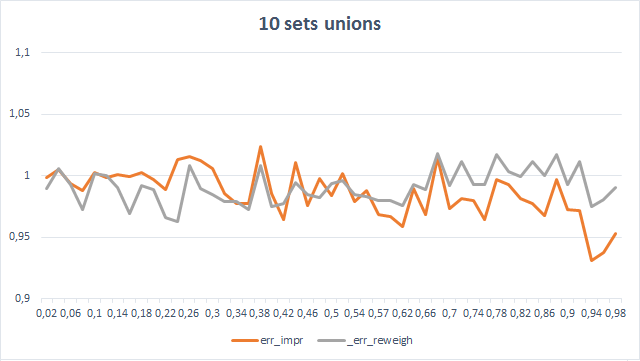
\includegraphics[width=0.6\textwidth]{KMV_10_sets_unions.png}
    \centering
    \caption{Porównanie metod dla sumy 10 zbiorów}
    \label{fig:KMV_10sets_unions}
\end{figure}

\begin{figure}[h!]
    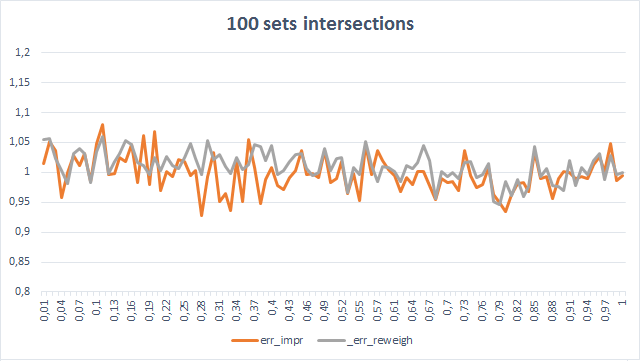
\includegraphics[width=0.6\textwidth]{KMV_100_sets_inter.png}
    \centering
    \caption{Porównanie metod dla przekroju 100 zbiorów}
    \label{fig:KMV_100sets_inter}
\end{figure}

\begin{figure}[h!]
    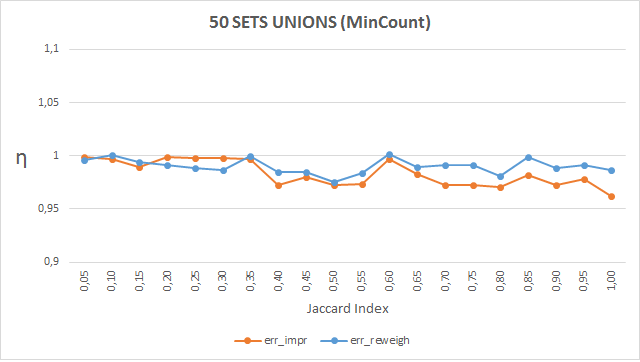
\includegraphics[width=0.6\textwidth]{KMV_100_sets_unions.png}
    \centering
    \caption{Porównanie metod dla sumy 100 zbiorów}
    \label{fig:KMV_100sets_unions}
\end{figure}

Ostatnimi eksperymentami przeprowadzonymi dla algorytmu \texttt{MinCount} było sprawdzenie metody \textit{estymatora ważonego} dla różnicy zbiorów, omówionej w rozdziale \ref{diff_weighted}. Na wykresie \ref{fig:KMV_2_sets_diff} przedstawiamy wyniki dla różnicy dwóch zbiorów, porównując podejście naiwne oraz podejście wykorzystujące \textit{estymator ważony}.

\begin{figure}[h!]
    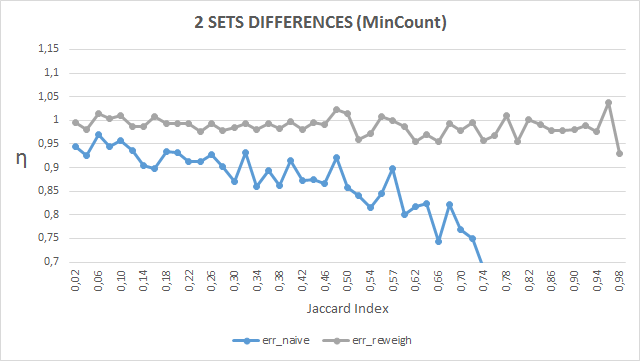
\includegraphics[width=0.6\textwidth]{KMV_2_sets_diff.png}
    \centering
    \caption{Porównanie metod dla różnicy 2 zbiorów}
    \label{fig:KMV_2_sets_diff}
\end{figure}

Zauważmy ze metody $2.$ oraz $3.$ po raz kolejny wypadają znacznie lepiej od metody naiwnej, a metoda \textit{estymatora ważonego}, podobnie jak w przypadku sumy i przekroju, pokrywa się z tendencją metody $2.$, ale w większości przypadków posiada mniejszy błąd.

\newpage
\section{Wyniki dla algorytmu HyperLogLog}
W tym podrozdziale przedstawimy wyniki dla algorytmu \texttt{HyperLogLog}. Zestawiliśmy ze sobą dwie metody:
\begin{enumerate}
	\item metoda naiwna z użyciem indeksu \textit{Jaccarda} (wzór (\ref{jacc_1}))
	\item metoda \textit{estymatora ważonego}
\end{enumerate}
Obydwie metody korzystają z pomocniczej struktury dla każdego ze szkiców, przechowującej $k$ najmniejszych wartości (czyli zasadniczo z podstawowej wersji szkicu \texttt{MinCount}), pozwalającej na estymację indeksu \textit{Jaccarda} \cite{adroll}, potrzebnego zarówno do estymacji metodą naiwną jak i metodą \textit{estymatora ważonego}. W przeprowadzanych eksperymentach ustaliliśmy parametry $k = 80$ oraz $p = 8$.
Na wykresach przedstawiamy wartości $\frac{\hat{n}}{n}$ dla poszczególnych metod, oznaczone na legendzie przez odpowiednio:
\begin{enumerate}
	\item \textbf{err\_naive}
	\item \textbf{err\_reweigh}
\end{enumerate}

Na wykresach \ref{fig:HLL_2_sets_unions}, \ref{fig:HLL_2_sets_unions}, \ref{fig:HLL_10_sets_unions} oraz \ref{fig:HLL_10_sets_inter} przedstawiamy porównanie powyższych metod w kontekście operacji sumy oraz przekroju. Eksperymenty przeprowadziliśmy dla 2 oraz 10 zbiorów o mocach $n=10^5$.

\begin{figure}[h!]
	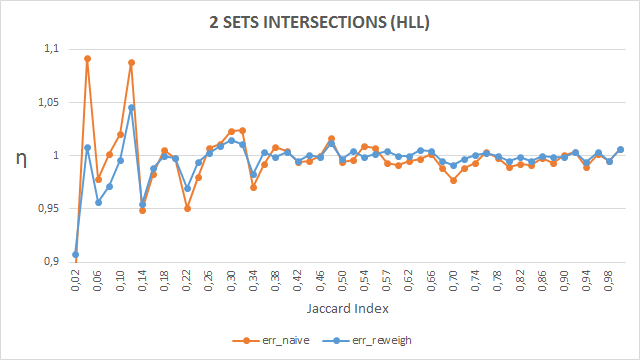
\includegraphics[width=0.6\textwidth]{HLL_2_sets_inter.png}
	\centering
	\caption{Porównanie metod dla przekroju 2 zbiorów przy $n=10^5$}
	\label{fig:HLL_2_sets_inter}
\end{figure}

\begin{figure}[h!]
	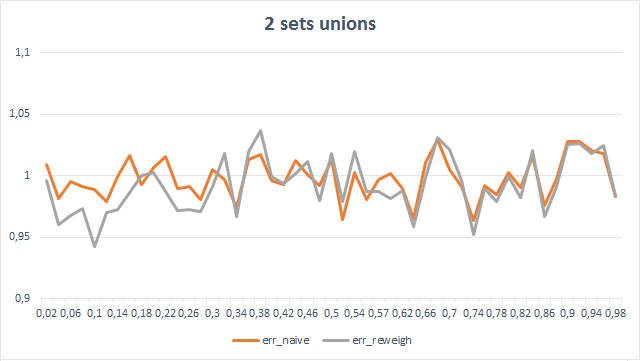
\includegraphics[width=0.6\textwidth]{HLL_2_sets_unions.png}
	\centering
	\caption{Porównanie metod dla sumy 2 zbiorów przy $n=10^5$}
	\label{fig:HLL_2_sets_unions}
\end{figure}

\begin{figure}[h!]
    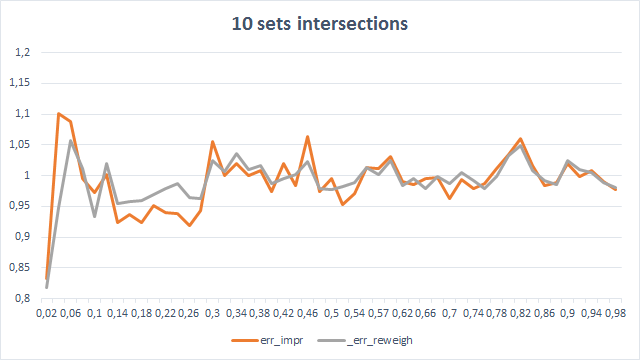
\includegraphics[width=0.6\textwidth]{HLL_10_sets_inter.png}
    \centering
    \caption{Porównanie metod dla przekroju 10 zbiorów przy $n=10^5$}
    \label{fig:HLL_10_sets_inter}
\end{figure}
\AW{tutaj jest blad w legendzie na wykresie - powinno byc err\_naive zamiast err\_impr!}

\begin{figure}[h!]
    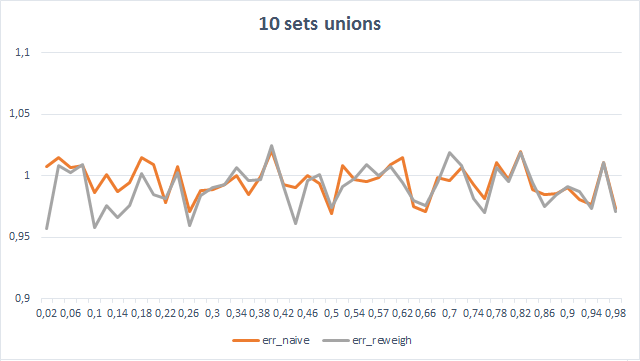
\includegraphics[width=0.6\textwidth]{HLL_10_sets_unions.png}
    \centering
    \caption{Porównanie metod dla sumy 10 zbiorów przy $n=10^5$}
    \label{fig:HLL_10_sets_unions}
\end{figure}

Wnioski wynikające z tych eksperymentów sugerują, że metoda \textit{estymatora ważonego} w kontekście algorytmu \texttt{HyperLogLog} dla operacji sumy niestety nie dorównuje pod względem dokładności podejściu naiwnemu. W przypadku sumy jest to dosyć oczywiste, ponieważ jak wspominaliśmy w rozdziale 2 - \texttt{HyperLogLog} posiada naturalną operację sumy. W przypadku operacji przekroju metoda naiwna wykorzystująca indeks \textit{Jaccarda} i wzór (\ref{jacc_1}) posiada większy błąd niż estymacja z użyciem \textit{estymatora ważonego}, zwłaszcza dla zbiorów o niskim podobieństwie. Zauważmy że obie metody wykorzystują tyle samo pamięci, bowiem obie wymagają dodatkowej struktury pozwalającej na estymację indeksu \textit{Jaccarda} przy wykorzystaniu algorytmu \texttt{MinHash}.